\subsection{The \texttt{FPSPH:} module}

The {\tt FPSPH:} module performs a single fixed-point (aka. Picard) or Newton SPH iteration. This module is intended to be used in
a {\tt REPEAT UNTIL} loop, implemented in CLE-2000 macro-language, where the macro calculation is explicitely called, as depicted
in Figs.~\ref{fig:fig_fpsph} and~\ref{fig:fig_fnewton}.

\vskip 0.2cm

\begin{figure}[h!]
\begin{center}
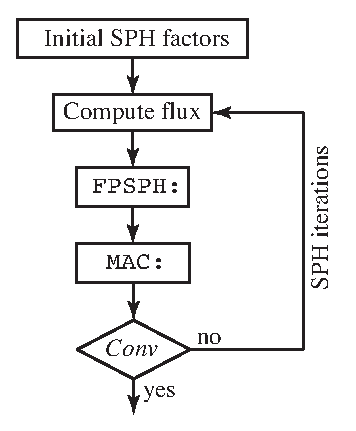
\includegraphics[scale=0.85]{Figures/fpsph.eps} 
\caption{Fixed point SPH iterations.}\label{fig:fig_fpsph}
\end{center}
\end{figure}

\begin{figure}[h!]
\begin{center}
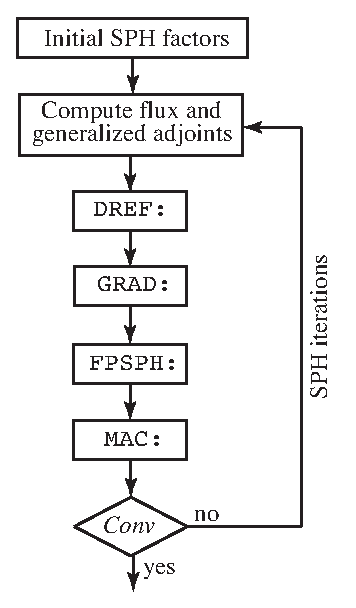
\includegraphics[scale=0.85]{Figures/flow_newton.eps} 
\caption{Newton SPH iterations.}\label{fig:fig_fnewton}
\end{center}
\end{figure}

\clearpage

The calling specifications are:

\begin{DataStructure}{Structure \moc{FPSPH:}}
\dusa{OPTIM} \moc{:=} \moc{FPSPH:} $[$ \dusa{OPTIM} $]$ \dusa{MACROLIB} \dusa{MACROREF} \moc{::} \dstr{fpsph\_data}
\end{DataStructure}

\noindent where

\begin{ListeDeDescription}{mmmmmmmm}

\item[\dusa{OPTIM}] \texttt{character*12} name of the \dds{optimize} object ({\tt L\_OPTIMIZE} signature) containing the
SPH factors. At the first call, object \dusa{OPTIM} must appear on LHS to receive its initial values. On subsequent calls, object
\dusa{OPTIM} must appear on both LHS and RHS to be able to update the previous values.

\item[\dusa{MACROLIB}] \texttt{character*12} name of the read-only extended \dds{macrolib} object ({\tt L\_MACROLIB} signature) containing the
macroscopic cross sections used by the macro-calculation and fluxes produced by the macro-calculation.

\item[\dusa{MACROREF}] \texttt{character*12} name of the read-only extended \dds{macrolib} object ({\tt L\_MACROLIB} signature) containing the
reference macroscopic cross sections and fluxes.

\item[\dstr{fpsph\_data}] structure containing the data to the module \texttt{FPSPH:} (see Sect.~\ref{sect:lnsr_data}).

\end{ListeDeDescription}
\vskip 0.2cm

\subsubsection{Data input for module \texttt{FPSPH:}}\label{sect:lnsr_data}

\begin{DataStructure}{Structure \moc{fpsph\_data}}
$[$ \moc{EDIT} \dusa{iprint} $]$ \\
$[~$\moc{SPH} $\{$ \moc{PN} $|$ \moc{SN} $\}~]$ \\
$[$ \moc{GRPMIN} \dusa{ngr1} $]~[$ \moc{GRPMAX} \dusa{ngr2} $]$\\
$[$ \moc{OUT-STEP-EPS} \dusa{$\epsilon_{ext}$} \\
$[$ \moc{VAR-VAL-MIN} \dusa{varmin} $]~[$ \moc{VAR-VAL-MAX} \dusa{varmax} $]$ \\
$[$ \moc{OUT-CONV-TST} {\tt >>} \dusa{$l_{conv}$} {\tt <<} $]$ \\
;
\end{DataStructure}

\noindent where
\begin{ListeDeDescription}{mmmmmmmm}

\item[\moc{EDIT}] keyword used to set \dusa{iprint}.

\item[\dusa{iprint}] index used to control the printing in module.

\item[\moc{PN}] keyword to activate a calculation of heterogeneous SPH factors of diffusion, PN or SPN type.

\item[\moc{SN}] keyword to activate a calculation of heterogeneous SPH factors of PIJ, IC, SN or MOC type.
This is the default option.

\item[\moc{GRPMIN}] keyword used to set the first energy group where SPH correction is applied. By default,
the first energy group index is used.

\item[\dusa{ngr1}] minimum energy group index where SPH correction is applied.

\item[\moc{GRPMAX}] keyword used to set the last energy group where SPH correction is applied. By default,
the total number of energy groups in \dusa{MACROLIB} is used.

\item[\dusa{ngr2}] maximum energy group index where SPH correction is applied.

\item[\moc{OUT-STEP-EPS}] keyword used to set the tolerance of SPH iteration convergence inside module {\tt FPSPH:} (default value
is $1.0 \times 10^{-4}$).

\item[\dusa{$\epsilon_{ext}$}] tolerance value (real or double precision).

\item[\moc{VAR-VAL-MIN}] keyword to specify the minimum values of the SPH factors. These values can also be set in a previous call
to module {\tt GRAD:}.

\item[\dusa{varmin}] single real value used for all SPH factors.

\item[\moc{VAR-VAL-MAX}] keyword to specify the maximum values of the SPH factors. These values can also be set in a previous call
to module {\tt GRAD:}.

\item[\dusa{varmax}] single real value used for all SPH factors.

\item[\moc{OUT-CONV-TST}] keyword used to determine if the SPH convergence has been reached.

\item[\dusa{$l_{conv}$}] $=1$ means that SPH convergence has been reached; $=0$ otherwise.

\end{ListeDeDescription}
\clearpage
